%!TEX program = xelatex
\documentclass[cn,hazy,black,10pt,normal]{elegantnote}
\usepackage{hyperref}
\usepackage{amssymb}
\usepackage[version=3]{mhchem}

% font settings
\definecolor{mgreen}{RGB}{0,166,82}
\definecolor{guess}{RGB}{47,79,79}
\newenvironment{guess}{
  \color{guess}}{\newline \color{black}}

% cover settings
\title{高中数学II习题集}

\author{Johnny Tang}
\institute{DEEP Team}

\date{\zhtoday}

% customised commands
\usepackage{ulem}
	\newcommand{\tk}{\uline{\hspace{4em}}}
\DeclareSymbolFont{yh}{OMX}{yhex}{m}{n}
\DeclareMathAccent{\hu}{\mathord}{yh}{"F3}
\newcommand{\xl}[1]{\overrightarrow{#1}}
\newcommand{\nd}[1]{〔#1〕}
\newcommand{\cor}{~\textit{或}~}
\newcommand{\ssb}[1]{\left( #1 \right)}
\newcommand{\sw}[1]{\boxed{\text{解法 #1}} \ }
\newcommand{\buzhou}[1]{$#1^{\circ} \ $}
\newcommand{\R}{\mathbb{R}}
\newcommand{\hlt}[1]{\color{red} #1 \color{black}}
\DeclareMathOperator{\card}{card}

% 行距设置
\setlength{\lineskiplimit}{5pt} %至少宽度
\setlength{\lineskip}{4pt} %正常宽度
\setlength{\normallineskiplimit}{5pt} %正常宽度
\setlength{\normallineskip}{5pt} %正常宽度


\begin{document}

\maketitle

\chapter{兴趣二阶代数}

\section{不等式中的恒等变形}

\subsection{整式变形}

\begin{proposition}{常见三元恒等变形公式}
	(1)$$a^3+b^3+c^3-3abc = (a+b+c)(a^2+b^2+c^2-ab-bc-ca)$$
	(2)$$(a+b)(b+c)(c+a) = a^2b + b^2c + c^2a + ab^2 + bc^2 + ca^2 +2abc$$
	(3)$$(a+b+c)(ab+bc+ca) = a^2b + b^2c + c^2a + ab^2 + bc^2 + ca^2 +3abc$$
	(4)$$(a-b)(b-c)(c-a) = \color{red}-\color{black}(a^2b+b^2c+c^2a)\color{red}+\color{black}(ab^2+bc^2+ca^2)$$
	(5)$$(a+b-c)(b+c-a)(c+a-b) = a^2b+b^2c+c^2a+ab^2+bc^2+ca^2-a^3-b^3-c^3-2abc$$
	(6)$$(a+b+c)(a+b-c)(b+c-a)(c+a-b) = 2a^2b^2 + 2b^2c^2 + 2c^2a^2 - a^4 -b^4-c^4$$
\end{proposition}

然而最近几年三元变形不太常考.

\begin{theorem}{Schur不等式}
	设实数$a,b,c,t$满足$a,b,c \geq 0$,则$$a^t(a-b)(a-c) + b^t(b-c)(b-a) + c^t(c-a)(c-b) \geq 0$$
	当且仅当$a,b,c$中有两个相等、另一个为$0$或$a=b=c$时取等.
\end{theorem}
\begin{proof}
	不妨设$a \geq b \geq c$,注意到$a-c=(a-b)+(b-c)$,所以
	\begin{align*}
		LHS &= a^t(a-b)^2 + a^t(a-b)(b-c) - b^t(b-c)(a-b) + c^t(b-c)^2 + c^t(a-b)(b-c) \\
		&= a^t(a-b)^2 + c^t(b-c)^2 + (a^t-b^t+c^t)(a-b)(b-c) \geq 0
	\end{align*}
\end{proof}

\begin{corollary}{反向的三元不等式形式}
	当$t=1$时,有$$a(a-b)(a-c) + b(b-c)(b-a) + c(c-a)(c-b) \geq 0$$
	即$$a^3+b^3+c^3+3abc \geq a^2b + b^2c + c^2a + ab^2 + bc^2 + ca^2$$
\end{corollary}
\begin{remark}
	这个不等式意义在于:$\sum ab(a+b)$放在较小的一侧,这是Cauchy/均值不等式等无法做到的.
\end{remark}

\begin{problem} % 兴趣二阶代数p8
	\nd{1}已知$a \geq b \geq c \geq 0$,证明:$$ab^2+bc^2+ca^2 \leq \frac{1}{8} (a+b+c)^3$$
\end{problem}
\begin{hint}
	将不对称的形式转化为对称处理.
\end{hint}
\begin{solution}
	由$-(a^2b+b^2c+c^2a)+(ab^2+bc^2+ca^2) = (a-b)(b-c)(c-a) \leq 0$,可知$$ab^2+bc^2+ca^2 \leq a^2b+b^2c+c^2a$$
	于是$$ab^2+bc^2+ca^2 \leq \frac{1}{2} (a^2b+b^2c+c^2a+ab^2+bc^2+ca^2)$$
	现在只需证明$$(a+b+c)^3 \geq 4(a^2b+b^2c+c^2a+ab^2+bc^2+ca^2)$$
	即$$a^3+b^3+c^3+6abc \geq a^2b+b^2c+c^2a+ab^2+bc^2+ca^2$$
	实际上,由$3abc \geq 0$与$a^3+b^3+c^3+3abc \geq a^2b + b^2c + c^2a + ab^2 + bc^2 + ca^2$,这个式子自然成立.
\end{solution}


\subsection{分式变形}

\begin{problem} % 兴趣二阶代数p7
	\nd{1}设$n$是正整数,$a_1,a_2, \cdots ,a_n$是非负实数,证明:$$\frac{1}{1+a_1} + \frac{a_1}{(1+a_1)(1+a_2)} + \cdots + \frac{a_1a_2 \cdots a_{n-1}}{(1+a_1)(1+a_2) \cdots (1+a_n)} \leq 1$$
\end{problem}
\begin{solution}
\begin{guess}
	观察左式形式,尝试进行通分操作.
	\begin{align*}
		&n=1, \quad \frac{1}{1+a_1} = 1 - \frac{a_1}{1+a_1} \\
		&n=2, \quad \frac{1}{1+a_1} + \frac{a_1}{(1+a_1)(1+a_2)} = \frac{1+a_1+a_2}{(1+a_1)(1+a_2)} = 1 - \frac{a_1a_2}{(1+a_1)(1+a_2)} \\
		&n=3, \quad \frac{1}{1+a_1} + \frac{a_1}{(1+a_1)(1+a_2)} + \frac{a_1a_2}{(1+a_1)(1+a_2)(1+a_3)} = 1 - \frac{a_1a_2a_3}{(1+a_1)(1+a_2)(1+a_3)}
	\end{align*}
	于是猜测$$LHS = 1 - \frac{a_1a_2 \cdots a_n}{(1+a_1)(1+a_2) \cdots (1+a_n)}$$
\end{guess}
	记$f(n) = LHS$,$g(n) = 1 - \dfrac{a_1a_2 \cdots a_n}{(1+a_1)(1+a_2) \cdots (1+a_n)}$. \\
	作$$\frac{a_1a_2 \cdots a_{n-1}}{(1+a_1)(1+a_2) \cdots (1+a_n)} + \frac{a_1a_2 \cdots a_n}{(1+a_1)(1+a_2) \cdots (1+a_n)} = \frac{(a_1a_2 \cdots a_{n-1})(1+a_n)}{(1+a_1)(1+a_2) \cdots (1+a_n)} = 1-g(n-1)$$
	即$f(n)-f(n-1) + 1-g(n) = 1-g(n-1)$.于是$f(n)-g(n) = f(n-1)-g(n-1)$. \\
	对$n$归纳证明$f(n)=g(n)$:当$n=1$时,$f(n) = \dfrac{1}{2} = g(n)$;假设当$n=k$时成立,即$f(n)=g(n)$,由上述等式可知$f(n+1)=g(n+1)$,于是当$n=k+1$时也成立.由数学归纳原理,$f(n)=g(n)$.故$$LHS = 1 - \frac{a_1a_2 \cdots a_n}{(1+a_1)(1+a_2) \cdots (1+a_n)} \leq 1$$
\end{solution}

\subsection{求和符号变形}

\begin{proposition}{常见求和符号变形公式}
	(1)$$\ssb{ \sum_{i=1}^{n} a_i }^2 = \sum_{i=1}^{n} a_i^2 + 2 \sum_{1 \leq i < j \leq n} a_ia_j$$
	(2)$$\ssb{ \sum_{i=1}^{n} a_i } \cdot \ssb{ \sum_{j=1}^{n} a_j } = \sum_{i=1}^{n} \ssb{a_i \cdot \sum_{j=1}^{n} a_j} = \sum_{i=1}^{n} \sum_{j=1}^{n} a_ib_j = \sum_{j=1}^{n} \sum_{i=1}^{n} a_ib_j$$
	(3)$$\sum_{1 \leq i < j \leq n} a_ia_j = \sum_{i=1}^{n-1} \sum_{j=i+1}^{n} a_ia_j = \sum_{j=2}^{n} \sum_{i=1}^{j-1} a_ia_j$$
\end{proposition}

\begin{problem} % 兴趣二阶代数p8
	\nd{1}设$2n$个实数$a_1,a_2, \cdots ,a_{2n}$满足条件$$\sum_{i=1}^{2n-1} (a_{i+1}-a_i)^2 = 1$$
	求$$(a_{n+1} + a_{n+2} + \cdots + a_{2n}) - (a_{1} + a_{2} + \cdots + a_{n})$$的最大值.
\end{problem}
\begin{hint}
	利用求和符号化简.
\end{hint}
\begin{solution}
	设$\{ b_n \}$满足$b_i = a_{i+1} - a_i$,由题可知$b_1^2 + \cdots + b_n^2 = 1$.由于$$S_0 = \sum_{i=1}^{n} (a_{n+i} - a_i) = \sum_{i=1}^{n} \sum_{j=i}^{n+i-1} b_j$$
	对于给定的$b_k$,满足$i \leq k \leq n+i-1$的$i$的个数就是最终$b_k$的系数.容易发现该个数为$$
	\begin{cases}
		k, \quad &k \leq n \\
		2n-k, & k \geq n
	\end{cases}$$
	于是$$S_0 = b_1+2b_2 + \cdots + (n-1)b_{n-1} + nb_n + (n-1)b_{n+1} + \cdots + b_{2n-1}$$
	由Cauchy不等式,可知
	\begin{align*}
		(S_0)^2 &\leq (b_1^2+b_2^2 + \cdots + b_{2n-1}^2)[2(1^2+2^2 + \cdots + (n-1)^2)+n^2] \\
		&= \frac{(n-1)n(2n-1)}{3} + n^2 = \frac{2n^3+n}{3}
	\end{align*}
	故$S_0 \leq \sqrt{\dfrac{2n^3+n}{3}}$,当且仅当$\dfrac{b_1}{1} = \cdots = \dfrac{b_n}{n} = \dfrac{b_{n+1}}{n-1} = \cdots = \dfrac{b_{2n-1}}{1}$时取等.
\end{solution}

\subsection{注重变形的不等关系}

\begin{problem} % 兴趣二阶代数p10
	\nd{1}设$x_1,~x_2,~y_1,~y_2,~z_1,~z_2$都是实数,且满足$x_1,~x_2,~x_1y_1-z_1^2,~x_2y_2-z_2^2 > 0$.证明:$$\frac{8}{(x_1+x_2)(y_1+y_2)-(z_1+z_2)^2} \leq \frac{1}{x_1y_1-z_1^2} + \frac{1}{x_2y_2-z_2^2} $$
	并指出等号成立的条件.
\end{problem}
\begin{solution}
	\begin{guess}
		记$S=\dfrac{8}{LHS}$,由于$$S = x_1y_1-z_1^2+x_2y_2-z_2^2+x_1y_2+x_2y_1-2z_1z_2$$
		可以得到一些直觉:(1)想要把$S$凑成$(\sqrt{x_1y_1-z_1^2} + \sqrt{x_2y_2-z_2^2})^2$的形式;(2)想要把$x_1y_2+x_2y_1$变得整齐一些.于是考虑利用均值不等式变形.
	\end{guess}
	由均值不等式,有
	\begin{align*}
		S &\geq x_1y_1-z_1^2+x_2y_2-z_2^2+2(\sqrt{x_1y_1x_2y_2}-z_1z_2) \\
		&= x_1y_1-z_1^2+x_2y_2-z_2^2+2\sqrt{x_1y_1x_2y_2 + (z_1z_2)^2 - 2(z_1\sqrt{x_2y_2}) \cdot (z_2 \sqrt{x_1y_1})} \\
		&\geq x_1y_1-z_1^2+x_2y_2-z_2^2+2\sqrt{x_1y_1 \cdot x_2y_2 + z_1^2z_2^2 - z_1^2x_2y_2 - z_2^2x_1y_1} \\
		&= x_1y_1-z_1^2+x_2y_2-z_2^2+2\sqrt{(x_1y_1-z_1^2)(x_2y_2-z_2^2)} \\
		&= (\sqrt{x_1y_1-z_1^2} + \sqrt{x_2y_2-z_2^2})^2
	\end{align*}
	其中,第一个不等式在$x_1y_2=x_2y_1$时取等,第二个不等式在$z_1^2x_2y_2=z_2^2x_1y_1$时取等. \\
	令$s=\sqrt{x_1y_1-z_1^2},~t=\sqrt{x_2y_2-z_2^2}$,只需证明$$\frac{8}{(s+t)^2} \leq \frac{1}{s^2} + \frac{1}{t^2}$$
	即要证明$(s^2+t^2+4st)(s-t)^2 \geq 0$.这是显然的,且该式在$s=t$即$x_1y_1-z_1^2=x_2y_2-z_2^2$时取等. \\
	另外,在原不等式取等时,有$$
	\begin{cases}
		x_1y_2=x_2y_1 \\
		z_1^2x_2y_2=z_2^2x_1y_1 \\
		x_1y_1-z_1^2=x_2y_2-z_2^2
	\end{cases}$$
	由第三个式子,可知$z_2^2=x_2y_2-x_1y_1+z_1^2$.带入第二个式子,解得$x_2y_2=x_1y_1$.与第一个式子相除,可解得$x_1=x_2,~y_1=y_2,~z_1=z_2$. \\
	综上,原不等式成立,且其取等条件为$x_1=x_2,~y_1=y_2,~z_1=z_2$.
\end{solution}

\section{齐次化}

\begin{problem} % 兴趣二阶代数p9
	\nd{1}设正实数$a,b,c$,满足$a+b+c=abc$.证明:$$\frac{1}{a^2+1} + \frac{1}{b^2+1} + \frac{1}{c^2+1} \geq \frac{3}{4}$$
\end{problem}
\begin{hint}
	齐次化处理.
\end{hint}
\begin{solution}
	由$a+b+c=abc$,有$\dfrac{abc}{a+b+c}=1$.于是$$LHS = \sum \frac{\dfrac{abc}{a+b+c}}{a^2 + \dfrac{abc}{a+b+c}} = \sum \frac{bc}{a^2+ab+ac+bc} = \sum \frac{bc}{(a+b)(a+c)}$$
	即只需证明$$4\sum ab(a+b) - 3\prod (a+b) \geq 0$$
	化简,即$$a^2b+ab^2+b^2c+bc^2+c^2a+ca^2 \geq 6abc$$
	由$a^2b+b^2c+c^2a \geq 0$与$ab^2+bc^2+ca^2 \geq 0$可知上式成立.于是原题证毕.
\end{solution}

\section{数学归纳法与数列变形}

\begin{problem} % 兴趣二阶代数p7
	\nd{1}证明:对任意的正整数,有$$\sqrt{1^2+ \sqrt{2^2+ \sqrt{3^2+ \cdots + \sqrt{n^2}}}}<2$$
\end{problem}
\begin{hint}
	尝试对$n$进行归纳证明.发现在$n=k+1$时,不等号方向不对,而证明加强命题比较麻烦,不如换个角度进行归纳.
\end{hint}
\begin{solution}
	设$a_m = \sqrt{m^2+\sqrt{(m+1)^2 + \cdots + \sqrt{n^2}}}$.于是$a_m=a_{m-1}^2-(m-1)^2$,且$a_n=n$,$a_1=LHS$. \\
	以下对$m$反向归纳证明$a_m<m+1$.当$m=n$时命题成立;假设$m=k$时命题成立,那么当$m=k-1$时,$$a_{k-1} = \sqrt{a_k + (k-1)^2} < \sqrt{k^2-k+2} \leq k$$
	其中$k \geq 2$.由归纳原理,$a_m<m+1~(m \geq 1)$,于是$LHS=a_1 <2$.
\end{solution}




\chapter{兴趣二阶组合}

\section{抽屉原理}

\begin{theorem}{抽屉原理}
	有$m$个小球,$n$个抽屉,那么存在一个抽屉放了至少$\left[ \dfrac{m-1}{n} \right]+1$个、至多$\left[ \dfrac{m}{n} \right]$个小球.
\end{theorem}
\begin{proof}
	(1)假设所有抽屉最多有$\left[ \dfrac{m-1}{n} \right]$个小球,则总小球数目至多为$$\left[ \frac{m-1}{n} \right] \times n \leq \frac{m-1}{n} \times n = m-1 < m$$
	这与条件矛盾. \\
	(2)假设所有抽屉至少有$\left[ \dfrac{m}{n} \right] + 1$个小球,则总小球数目至少为$$\ssb{\left[ \dfrac{m}{n} \right] + 1} \times n > \frac{m}{n} \times n = m$$
	这与条件矛盾.
\end{proof}

\begin{corollary}{平均值原理}
	对于给定的实数$a_1, \cdots ,a_n$,存在$a_i,a_j$使得$$a_i \geq \dfrac{1}{n}(a_1+ \cdots +a_n), \quad a_j \leq \dfrac{1}{n}(a_1+ \cdots +a_n)$$
\end{corollary}

\begin{problem} % 兴趣二阶组合1.1
	\nd{1}证明: \\
	(1)从前$100$个正整数中任意取出$51$个数,都可以找到两个数,使得它们中的一个是另一个的整数倍. \\
	(2)从前$91$个正整数中任意取出$10$个数,则一定有两个数,使得这两个数中较大数不超过较小数的$1.5$倍. \\
	(3)若$a_1,a_2,\cdots ,a_{100}$都是实数,且在集合$\{ a_1, \dfrac{a_1+a_2}{2}, \cdots ,\dfrac{a_1+a_2+\cdots +a_{100}}{100} \}$中至少有$51$个元素的值相等,则$a_1,a_2, \cdots ,a_{100}$中有两个数相等.
\end{problem}
\begin{solution}
	(1)构造:$$\{ 1 \times 2^0, \cdots , 1 \times 2^6 \},\{ 3 \times 2^0, \cdots , 3 \times 2^5 \}, \cdots ,\{99 \times 2^0 \}$$共$50$个抽屉.由抽屉原理,在前$100$个正整数中必有两个数在同一个抽屉中,即它们有倍数关系. \\
	(2)构造:$$\{ 1 \},\{ 2,3 \},\{ 4,5,6 \},\{ 7,8,9,10 \},\{ 11,12,13,14,15,16 \},\{ 17,\cdots 25 \},\{ 26,\cdots ,39 \},\{ 40, \cdots ,60 \},\{ 61, \cdots ,91 \}$$共$9$个抽屉.由抽屉原理,前$91$个正整数中必有两个在同一抽屉中,即满足较大数不超过较小数的$1.5$倍. \\
	(3)记$b_i=\dfrac{a_1+ \cdots + a_i}{i}$,注意到,若$b_i=b_{i+1}=p$,则$$\frac{a_1+ \cdots + a_i}{i} = \frac{a_1+ \cdots + a_i + a_{i+1}}{i+1}$$可得$a_{i+1} = \dfrac{a_1 + \cdots + a_i}{i} = b_i = p$.设$b_1, \cdots ,b_{100}$中相等的$51$个数均等于$p$. \\
	\buzhou{1} 当$a_1 \neq p$时:构造$$\{ b_1,b_2 \}, \cdots ,\{ b_{99},b_{100} \}$$共$50$个抽屉,同理存在$a_{2k+1}=p$;构造$$\{ b_2,b_3 \}, \cdots ,\{ b_{98},b_{99} \},\{ b_{100} \}$$共$50$个抽屉,同理存在$a_{2l}=p$.故$a_{2k+1}=a_{2l}$. \\
	\buzhou{2} 当$a_1=p$时:构造$$\{ b_2,b_3 \}, \cdots ,\{ b_{98},b_{99} \},\{ b_{100} \}$$共$50$个抽屉.由抽屉原理,必存在$b_{2k}=b_{2k+1}=p$,因而$a_{2k}=p=a_1$.
\end{solution}

\begin{problem} % 兴趣二阶组合1.2
	\nd{1}证明: \\
	(1)平面上任作$8$条互不平行的直线,其中必有两条直线的夹角小于$23$度. \\
	(2)给定一个由$10$个互不相等的两位十进制正整数组成的集合,则这个集合必有两个无公共元素的非空子集合,它们的元素和相等. \\
	(3)$100$个孩子围成一圈,其中$41$个男孩,$59$个女孩.则一定有$2$个男孩,他们中间的孩子个数恰为$19$的整数倍.
\end{problem}
\begin{solution}
	(1)由于平面上两直线的夹角不会随平移而改变,不妨平移这$8$条线使得它们交于同一点.由平均值原理,必有两条直线的夹角小于等于$22.5$度,即小于$23$度. \\
	(2)由于所有可能的非空子集个数为$2^{10}-1$,而子集和的所有可能情况只有在$[10,945]$中(共$936$种),由抽屉原理,必有两个子集的和相同. \\
	若这两个子集交集为空,则符合题意;若交集不空,则分别去掉交集中的元素,构成两个新的元素和相等且交集为空的集合. \\
	(3)假设这$100$个孩子的编号分别为$1, \cdots ,100$,则构造$$\{ 1,21,41,61,81 \}, \{ 2,22,42,62,82 \}, \cdots ,\{ 20,40,60,80,100 \}$$
	共$20$个集合.由抽屉原理,至少有一个集合中同时有三个男孩,即满足题意.
\end{solution}

\begin{problem} % 兴趣二阶组合1.3
	\nd{1}证明: \\
	(1)已知$a_1, \cdots a_{21}$是区间$(0,400)$内的$21$个实数,总可以找到两个数$a_i,a_j(1 \leq i < j \leq 21)$,满足$a_i+a_j < 1+2\sqrt{a_ia_j}$. \\
	(2)已知实数$0<a_1 < \cdots < a_{2011}$,则存在两个数$a_i,a_j(1 \leq i < j \leq 2011)$,满足$a_j-a_i < \dfrac{(1+a_i)(1+a_j)}{2010}$.
\end{problem}
\begin{solution}
	(1)只需证明$\sqrt{a_i}-\sqrt{a_j}<\sqrt{2}$即可.实际上,不妨设$a_1<\cdots <a_{21}$,那么在$\sqrt{a_{21}}-\sqrt{a_{20}}, \cdots ,\sqrt{a_2}-\sqrt{a_1}$中,由于它们的和为$\sqrt{a_{21}}-\sqrt{a_1} < 20$,由平均值原理可知其中必有一个$<1<\sqrt{2}$. \\
	(2)只需证明$\dfrac{1}{1+a_i}-\dfrac{1}{1+a_j} < \dfrac{1}{2010}$.与(1)同理可知.
\end{solution}

\begin{problem} % 兴趣二阶组合1.4
	\nd{1}从$4$个同心圆的圆心出发的$100$条射线等分各圆周,分别与$4$个圆各有$100$个交点.任意给每个圆上的点染上黑、白两色之一,使每个圆上都恰有$50$个黑点和$50$个白点.证明:可将此$4$个圆适当旋转,使这$100$条射线中至少存在$13$条射线,它们中的每一条穿过的$4$个点颜色都相同.
\end{problem}
\begin{hint}
	算两次.
\end{hint}
\begin{solution}
	对于给定的两个同心圆,设所有的组合方法为$P_1, \cdots ,P_{100}$,设第$i$种方法产生同色对个数$S(P_i)$. \\
	对于一条固定的射线,它经过一个同色对的方法数为$50$.由于共$100$条射线,可知$$S(P_1) + \cdots + S(P_{100}) = 100 \times 50 = 5000$$
	故由抽屉原理,存在一个$n$使得$S(P_n) \geq 50$.第一、二圈选择这样的方法,考虑新增的第三圈,设它与前两圈的组合方法为$Q_1, \cdots ,Q_{100}$,第$i$种方法产生同色组个数为$S(Q_i)$. \\
	对于一条穿过第一圈、第二圈上某个同色对的射线,它经过一个同色组的方法数为$50$.由于共$50$条这样的射线,可知$$S(Q_1) + \cdots + S(Q_{100}) = 50 \times 50 = 2500$$
	由抽屉原理,存在一个$m$使得$S(P_n) \geq 25$.同理,增加第四圈时至少有$\lceil 12.5 \rceil = 13$条射线穿过同色组,此即得证.
\end{solution}

\begin{problem} % 兴趣二阶组合1.5
	\nd{1}(1)设$S$为$\{ 1,2, \cdots ,n \}$的一个非空子集,满足其中任两个元素之和不为$n$,试求$|S|$的最大值. \\
	(2)从数$1,2,3, \cdots ,2017$中删去一些数,使得剩下的数中任何一个数都不等于其余任意两个不同的数的积,问最少要删去多少个数才能做到这一点?
\end{problem}
\begin{solution}
	(1)构造:$$\{ 1,n-1 \},\{ 2,n-2 \}, \cdots , \{ \left[ \frac{n}{2} \right], n-\left[ \frac{n}{2} \right] \},\{ n \}$$
	共$ \left[ \dfrac{n}{2} \right]+1$个抽屉.由抽屉原理,$|S| \leq \left[ \dfrac{n}{2} \right]+1$.例如,在$S = \{ 1,2, \cdots , \left[ \dfrac{n}{2} \right] ,n \}$时可以取到等号. \\
	(2)\begin{guess}
		保留$1,45 \sim 2017$可满足题意,即要构造$43$个抽屉.
	\end{guess}
	构造:$$\{ 44,45,44 \times 45 \}, \{ 43,46,43 \times 46 \}, \cdots , \{ 2,87,2\times 87 \}$$
	共$43$个抽屉.由抽屉原理,至少要去掉$43$个数才能保证不存在一个抽屉的所有元素都保留.例如,去掉$2 \sim 44$即可符合题意.
\end{solution}

\begin{problem} % 兴趣二阶组合1.6
	\nd{2} 若正整数集$S$中存在两个元素(可以相同)的和为$2$的幂,则称集$S$为\textit{优集};否则称为\textit{劣集}.求正整数$n$,使得$\{ 1,2,\cdots ,n \}$有一个含$99$个元素的\textit{劣集},而所有含$100$个元素的子集为\textit{优集}.
\end{problem}
\begin{hint}
	不妨换个方向:考虑对于给定的集合$\{ 1,2, \cdots ,n \}$,求它最大劣集的元素个数.
\end{hint}
\begin{solution}
	先考虑一个“基准”,即$n=2^k$时的情况.构造$$\{ 1,2^k-1 \}, \cdots ,\{ 2^{k-1}-1,2^{k-1}+1 \}$$
	共$2^{k-1}-1$个抽屉.若取原集合其中的$2^{k-1}$个数,要么每个抽屉取一个之后取到$2^{k-1}~ \textit{或} ~2^k$,要么(由抽屉原理)存在一个抽屉中有两个数.这显然是不符合要求的,因此最大劣集的元素个数为$2^{k-1}-1$,例如,$\{ 2^k-1, \cdots ,2^{k-1}+1 \}$就是一个这样的劣集. \\
	注意到,若$n=2^k-1$,所有情况与$n=2^k$是一样的.若设最大劣集的元素个数为$f(n)$,则有
	\begin{equation}
		f(2^{k}-1)= f(2^k)=2^{k-1}-1 \quad (k \geq 1)\label{erjp161}
	\end{equation}
	接着考虑一般情况,即$n=2^k+l~(1 \leq l \leq 2^{k+1}-2)$时.构造$$\{ 2^k-l,2^k+l \}, \cdots ,\{ 2^k-1,2^k+1 \}$$
	共$l$个抽屉.由抽屉原理,对于这$l$个抽屉,每个抽屉至多取一个元素.另外,若已取$2^k+1 , \cdots ,2^k+l$,对于$1, \cdots ,2^k-l-1$,可以取其中能构成劣集的元素.综上,
	\begin{equation}
		f(2^k+l)=f(2^k-l-1)+l \quad (1 \leq l \leq 2^{k+1}-2) \label{erjp162}
	\end{equation}
	综合式\ref{erjp161}与\ref{erjp162},可知$$f(2^k+l)=f(2^k-l-1)+l \quad (0 \leq l \leq 2^{k}-1)$$
	作以下估计:
	\small
	$$f(128)=65 \qquad f(256)=129$$
	$$f(200)=f(2^7+72)=f(55)+72=f(2^5+23)+72=f(8)+95=f(2^3)+95=97$$
	$$f(201)=f(2^7+73)=f(54)+73=f(2^5+22)+73=f(9)+95=f(2^3+1)+95=f(6)+96=f(2^2+2)+96=f(2)+98=98$$
	$$f(202)=f(2^7+74)=f(53)+74=f(2^5+21)+74=f(10)+95=f(2^3+2)+95=f(5)+97=f(2^2+1)+97=f(2)+98=98$$
	$$f(203)=f(2^7+75)=f(52)+75=f(2^5+20)+75=f(11)+95=f(2^3+3)+95=f(4)+98=99$$
	$$f(204)=f(2^7+76)=f(51)+76=f(2^5+19)+76=f(12)+95=f(2^3+4)+95=f(3)+99=100$$
	\normalsize
	于是$n=203$是满足题意的一个数.另一方面,容易证明$f(x)$是单调不减的函数(由劣集的定义),于是$n=203$是满足题意的唯一一个数.
\end{solution}

\begin{problem} % 兴趣二阶组合1.7
	\nd{1}(1)任选$6$人,试证:其中必有$3$人,他们互相认识或都不认识. \\
	(2)$17$名科学家中每两名科学家都进行了通信,而且任意两名科学家通信时只讨论三道题目中的一道题目.证明:至少有三名科学家,他们相互通信时讨论的是同一个题目.
\end{problem}
\begin{solution}
	(1)设这$6$个人$A_1, \cdots ,A_6$.考虑$A_1$与其他人的关系:把与$A_1$认识/不认识两种状态分别视作抽屉,由抽屉原理,至少存在一种状态有三个人满足.不妨设$A_1$与$A_2,A_3,A_4$互相认识. \\
	若$A_2,A_3,A_4$中有两人互相认识,则这两个人与$A_1$互相认识,符合题意;若$A_2,A_3,A_4$互不认识,也符合题意. \\ 
	综上,原命题得证. \\
	(2)考虑其中选定的一个人$A$.将三道题目分别视作抽屉,由抽屉原理,存在一道题被$A$与其他至少$6$人讨论,记此题为$1$号题,$A$与$A_1, \cdots ,A_6$讨论这道题. \\
	若$A_1, \cdots ,A_6$中有两人之间也讨论$1$号题,符合题意;若他们之中全不讨论$1$号题,不妨考虑$A_1$.将其余两道题目分别视作抽屉,由抽屉原理,存在一道题被$A_1$与其他至少$3$人讨论.记此题为$2$号题,不妨设这$3$人是$A_2,A_3,A_4$. \\
	若$A_2,A_3,A_4$中有两人讨论$2$号题,则符合题意;若他们之间全不讨论$2$号题,则他们之间必定互相讨论$3$号题,也符合题意. \\
	综上,原命题得证.
\end{solution}

\begin{problem} % 兴趣二阶组合1.8
	\nd{1}$300$名选手参加一次比赛,每两名选手或互相认识,或互不认识.已知没有三名选手两两认识,且每名选手至多认识其他$n$名选手.对于每个正整数$m~(1 \leq m \leq n)$,至少存在一名选手恰认识$m$名选手.求$n$的最大值.
\end{problem}
\begin{solution}
	\buzhou{1}证明有上界:考虑恰认识$n$个人的$A$.记所有$A$认识的人构成集合$S$,$A$不认识的人构成集合$T$,那么$|S|=n,~|T|=299-n$. \\
	由于没有三名选手两两认识,故$S$中没有两个互相认识的人,即$S$中的人只能认识$A$与$T$中的人,那么$S$中认识人最多的那个人最多只能认识$300-n$个人.假设$n$足够大,则恰认识$301-n, \cdots ,n-1$个人的人只能在$T$中,所以有$$299-n \geq (n-1) - (301-n) + 1$$
	这意味着$n \leq 200$. \\
	\buzhou{2}证明上界可取:取$n=200$,设$S$中的人分别为$B_1, \cdots , B_{100}$,$T$中的人分别为$A_1, \cdots ,A_{99}$. \\
	按如下规则构造即可:$A$认识所有$B_i$,$A_j$认识除$B_1 \sim B_{j}$之外的所有$B_i$,如下图所示:
	\begin{center}
		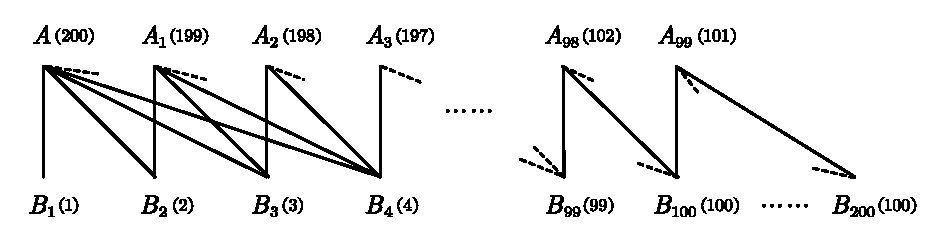
\includegraphics[width=14cm]{attachment/20230207.pdf}
	\end{center}
\end{solution}

\section{极端原理与无穷递降法}

\begin{instance}
	证明$\sqrt{2} \notin \mathbb{Q}$.
\end{instance}
\begin{solution}
	\begin{guess}
		设$\sqrt{2}=\dfrac{p}{q}$,则$q^2=2p^2$\ce{->T[令$q=2q_1$]}$2q_1^2=p^2$\ce{->T[令$p=2p_1$]}$2p_1^2=q_1^2 \cdots$然而不能像这样无穷递降下去.
	\end{guess}
	假设$(p,q)$是满足$q^2=2p^2$且使得$p+q$最小的一组数,若令$q=2q_1$,则$p^2=2q_1^2$,故$(q_1,p)$也满足要求,然而$q_1+p<p+q$,这与假设矛盾,故不存在满足要求的一组数.
\end{solution}

\begin{problem} % 兴趣二阶组合2.1
	\nd{1}已知对于任意$n$个互不相同的实数两两求和有$\dfrac{n(n-1)}{2}$种不同的求法.求正整数$n$,满足存在$n~(n \geq 3)$个互不相同的整数,使得这些数两两求和恰可构成$\dfrac{n(n-1)}{2}$个连续的正整数.
\end{problem}
\begin{solution}
	\buzhou{1}证明有上界:不妨设这$n$个数满足$a_1< \cdots <a_n$,于是$a_1+a_2<a_1+a_3< \textit{something} <a_{n-2}+a_n<a_{n-1}+a_n$.这意味着$a_3-a_2=1,~a_{n-1}-a_{n-2}=1$.若$n-2>3$,则必有$a_2+a_{n-1} = a_3+a_{n-2}$,因此$n \leq 5$. \\
	\buzhou{2}证明上界内部分可取:当$n=5$时,有$a_3-a_2=1,~a_4-a_3=1$,因而$$a_1+a_2 < a_1+a_3 < a_1+a_4 < \textit{something} < a_1+a_5 < \textit{something} <a_2+a_5 < a_3+a_5 < a_4+a_5$$
	其中两个\textit{something}的位置可以选择其一放置$a_2+a_3 < a_2+a_4 < a_3+a_4$.于是可知$(a_4+a_5) - (a_1+a_4)=7$,即$a_5-a_1=7$. \\
	若放在第一个位置,可得$a_2+a_3=a_1+a_4+1,~a_1+a_5=a_3+a_4+1$,解得$a_5=a_1+8$,矛盾; \\
	若放在第二个位置,可得$a_2+a_3=a_1+a_5+1,~a_2+a_5=a_3+a_4+1$,解得$a_5=a_1+8$,矛盾. \\
	因此,$n=5$时不合题意. \\
	另一方面,容易验证,当$n=3,4$时分别取
	$$(a_1,a_2,a_3) = (a_1,a_1+1,a_1+2)$$
	$$(a_1,a_2,a_3,a_4) = (a_1,a_1+1,a_1+2,a_1+4)$$
	可符合题意.综上,$n=3~ \textit{或} ~4$.
\end{solution}

\begin{problem} % 兴趣二阶组合2.2
	\nd{1}平面上有$n$个点,其中任三个点都可组成三角形,且面积均不超过$1$.证明:存在一个面积不超过$4$的三角形,它能覆盖住所有$n$个点.
\end{problem}
\begin{solution}
	设$\vartriangle ABC$是最大面积的三角形,分别过其中一个顶点作对边的平行线,记三条平行线交出三角形$\vartriangle A'B'C'$.任取新的一点.对于点$A,B$,由于所产生的三角形面积不超过$\vartriangle ABC$,故新的点一定在直线$A'B'$以上.同理该点在$B'C'$以下、$A'C'$以上,即其一定在三角形$\vartriangle A'B'C'$内.又$S_{\vartriangle A'B'C'} = 4S_{\vartriangle ABC} \leq 4$,故该三角形就是题目所求.
	\begin{center}
		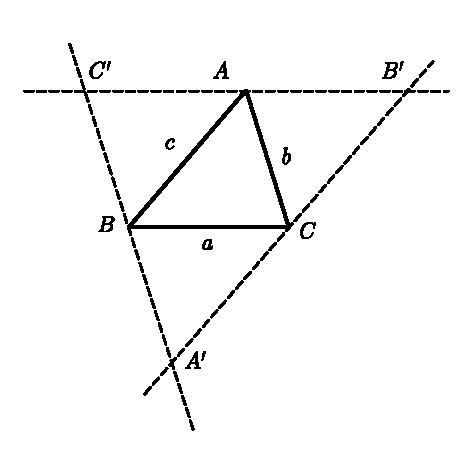
\includegraphics[width=6cm]{attachment/202302071.pdf}
	\end{center}
\end{solution}

\begin{problem} % 兴趣二阶组合2.3
	\nd{1}有$n$名($n \geq 3$)选手参加的一次乒乓球循环赛中,没有一个全胜的.问:能否找到三名选手$A,B,C$,使得$A$胜$B$,$B$胜$C$,$C$胜$A$?
\end{problem}
\begin{solution}
	设$A$是胜场最多的人.设所有败于$A$的人构成集合$X$,所有胜于$A$的人构成集合$Y$.若$Y$中的人全部胜于$X$中的人,则$Y$中任意一个人的胜场都比$A$多,这产生了矛盾.故存在$X$中的一个人胜于$Y$中的一个人,即符合题意.
\end{solution}

\begin{problem} % 兴趣二阶组合2.4
	\nd{1}已知$n~(n \geq 3)$名选手参加到一个循环赛.每名选手均有一个由数字$1$到$n$的等级,任意两名选手等级不一样.当$i < j$时,等级为$i$的选手总能打赢等级为$j$的选手.为了让比赛更有观赏性,组委会决定任意两名选手的比赛均由剩下的其他选手作为裁判来判决,每名裁判判决获胜者得$1$分,失败者得$0$分.最终,把所有裁判的加分相加即为每名选手的得分.当一名选手作为裁判时,他可以\textit{欺骗}得分,即输者给$1$分,嬴者$0$分.但他\textit{欺骗}的次数不能超过其等级数.求$n$的最大值,使得有可能让最弱的选手获得第一.
\end{problem}
\begin{solution}
	容易发现,当完全不发生欺骗时,$1$号选手分数为$(n-1)(n-2)$,$n$号选手分数为$0$.为了让$n$号的分数超过$1$号,需要$$2(n-2)+\left[ \frac{n(n+1)}{2} - (n-2) \right] \geq (n-1)(n-2)+1$$
	由此解得$\dfrac{9-\sqrt{41}}{2} \leq n \leq \dfrac{9+\sqrt{41}}{2}$.故$n \leq 7$. \\
	例如,在$n=7$时,如下欺骗可以达到效果:(其中黑体表示实行欺骗的选手,红体表示最终得分)
	
	\begin{table}[h]
	\centering
	\renewcommand\arraystretch{1.3}
\begin{tabular}{|l|l|l|l|l|l|l|l|l|}
\hline
    & $1$         & $2$         & $3$       & $4$     & $5$   & $6$   & $7$         & $\sum$ \\ \hline
$1$ & /           & $7~~\hlt{4}$         & $7~~\hlt{4}$       & $7~~\hlt{4}$     & $7~~\hlt{4}$   & $6,7~~\hlt{3}$ & $2,3,4,5,6~~\hlt{0}$ & $\hlt{19}$   \\ \hline
$2$ & $7~~\hlt{1}$         & /           & $\hlt{5}$          & $\hlt{5}$        & $7~~\hlt{4}$   & $7~~\hlt{4}$   & $1,3,4,5,6~~\hlt{0}$ & $\hlt{19}$   \\ \hline
$3$ & $7~~\hlt{1}$         & $\hlt{0}$            & /         & $\hlt{5}$        & $\hlt{5}$      & $\hlt{5}$      & $2,4,5,6~~\hlt{1}$   & $\hlt{17}$   \\ \hline
$4$ & $7~~\hlt{1}$         & $\hlt{0}$            & $\hlt{0}$          & /       & $\hlt{5}$      & $\hlt{5}$      & $3,5,6~~\hlt{2}$     & $\hlt{13}$   \\ \hline
$5$ & $7~~\hlt{1}$         & $7~~\hlt{1}$         & $\hlt{0}$          & $\hlt{0}$        & /     & $\hlt{5}$      & $4,6~~\hlt{3}$       & $\hlt{10}$   \\ \hline
$6$ & $6,7~~\hlt{2}$       & $7~~\hlt{1}$         & $\hlt{0}$          & $\hlt{0}$        & $\hlt{0}$      & /     & $5~~\hlt{4}$         & $\hlt{8}$    \\ \hline
$7$ & $2,3,4,5,6~~\hlt{5}$ & $1,3,4,5,6~~\hlt{5}$ & $2,4,5,6~~\hlt{4}$ & $3,5,6~~\hlt{3}$ & $4,6~~\hlt{2}$ & $5~~\hlt{1}$   & /           & $\hlt{20}$   \\ \hline
\end{tabular}
\end{table}
\end{solution}

\begin{problem} % 兴趣二阶组合2.5
	\nd{2}对于五元整数组,若其元素可以按某种顺序标记为$a,b,c,d,e$,使得$a-b+c-d+e=29$,则称此整数组为\textit{可安置的}.确定所有$2017$元整数组$(n_1,n_2, \cdots ,n_{2017})$,满足:若将这$2017$个数依次按顺时针方向放在圆周上($n_{2017}$与$n_1$相邻),则处于圆周上连续相邻位置的任一五元数组是\textit{可安置的}.
\end{problem}
\begin{solution}
	\begin{guess}
		在$n_i$全为$29$时明显符合题意,于是考虑证明这是唯一的情况.以下先乱写一通找找规律:
	\end{guess}
	对于$n_i$,由于$a-b+c-d+e=29$,可知$$a+b+c+d+e=29-2(b+d) \equiv 1\mod 2$$
	故连续$5$个数之和是奇数.由于$n_i+ \cdots + n_{i+4}$与$n_{i+1} + \cdots + n_{i+5}$都是奇数,知$n_i$与$n_{i+5}$同奇偶.注意到$(5,2017)=1$,由Bézout定理,所有$n_j$都与$n_i$同奇偶,又$a+b+c+d+e$为奇数,可知$$n_1 \equiv \cdots \equiv n_{2017} \equiv 1 \mod 2$$
	\begin{guess}
		这里的条件与奇偶性相关,可以尝试构造一直除以二的操作,说明最后总会除成奇数与一直是偶数矛盾.
	\end{guess}
	作变换$m_i=n_i-29$.于是$m_i$是偶数,并且对于$m_i$,条件转化为$$a' - b' + c' - d' + e' = \frac{a-29}{2} - \frac{b-29}{2} + \frac{c-29}{2} - \frac{d-29}{2} + \frac{e-29}{2} = 0$$
	注意到,将所有$m_i$除以二得到的新数组也满足$m_i$的性质,并且由这个性质可以推出任意$m_i$为偶数.然而,若$m_i \neq 0$,最后总会得到某个奇数,这是矛盾的.故$m_i=0$,即只有$n_1 = \cdots = n_{2017}=29$符合题意.
\end{solution}

\begin{problem} % 兴趣二阶组合2.6
	\nd{1}$E$是平面上$2n$个点构成的集合,其中任意三点不共线.现将其中$n$个点涂成红色,$n$个涂成蓝色.试证:总可找到两两没有公共点的$n$条线段,使其中每条线段的两个端点不同色.
\end{problem}
\begin{solution}
	\begin{guess}
		对于任意两条两端点不同色的线段,若它们有交点,则依照下列方式拆开.注意到这样拆开后两条线段的总长度严格变小,肯定会有一个停止的点.
	\end{guess}
	对于一种由红蓝点构成“两端点不同色”的线段的方法$p$,记所有这样线段的总长度为$s(p)$. \\
	考虑最小的$s(p)$及其对应的配对方式$p$.假设存在两条有交点的这样的线段,进行如下图所示操作,得到一种新的配对方式$p'$.因为三角形任两边之和大于第三边,可知$s(p')<s(p)$.这与条件矛盾,故由$p$配对得到的$n$条线段两两不相交.
	\begin{center}
		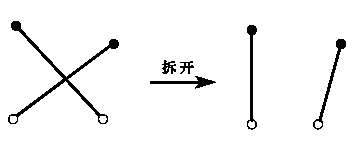
\includegraphics[width=6cm]{attachment/202302072.pdf}
	\end{center}
\end{solution}

\begin{problem} % 兴趣二阶组合2.7
	\nd{1}一次聚会中,每四个人中均存在三个人要么认识,要么不认识,认识是相互的.证明:将参加聚会的所有人分在两个房间内,使得一个房间中的人均互相认识,在另一个房间中没有一个人认识其他人.
\end{problem}
\begin{solution}
	设$A$是满足内部互相认识的最大房间,其中有$a_1, \cdots ,a_m$这些人;剩下的人$b_1, \cdots ,b_n$组成$B$. \\
	\buzhou{1}若$B$中只有一个人,自然原命题成立. \\
	\buzhou{2}若$B$中有多于一个人,不失一般性,假设$b_1$认识$b_2$.由于$A$是最大的满足条件的房间,在$A$中必有人不认识$b_1$与$b_2$,分两种情况讨论(不失一般性地): \\
	设$a_1$不认识$b_1$,$a_2$不认识$b_2$,如图$1$所示.这四个人的关系与题目条件矛盾; \\
	设$a_1$不认识$b_1$与$b_2$,任取$a_i \in A$考虑,如图$2$所示.若要满足题目条件,必有$a_i$认识$b_1$与$b_2$,这意味着任意的$a_i \in A$都认识$b_1$与$b_2$,故$b_1$与$b_2$也在$A$中,与$A$的性质矛盾. \\
	综上,假设不成立,即$B$中所有人都互不认识.
	\begin{center}
		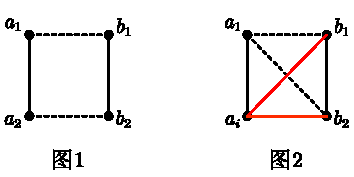
\includegraphics[width=5cm]{attachment/202302073.pdf}
	\end{center}
\end{solution}

\begin{problem} % 兴趣二阶组合2.8
	\nd{1}某届象棋比赛共有$64$名选手参赛.每两名选手赛一场(允许平局).所有比赛结束后,已知对所有以平局结束的比赛双方,剩余的$62$名选手均至少战胜过这两名选手之一,且至少有两场比赛以平局结束.证明:可将所有的选手排成一列,使得每名选手战胜过他后面的那一位选手.
\end{problem}
\begin{solution}
	\begin{guess}
		我们希望找到一个最长的链条$A_1 \to \cdots \to A_n$,当$n=64$时,题目结论即成立.
	\end{guess}
	假设存在最长的一个链条$A_1 \to \cdots \to A_n~(n < 64)$.设在此链条之外还有元素$B$. \\
	\buzhou{1}若$A_1, \cdots ,A_n$与$B$之间没有平局,如图$1$所示.由于$A_1$必战胜$B$(否则$B$就在链条的第一个),可知$B$不能战胜$A_2, \cdots ,A_n$(否则就会产生一个更长的链条),于是$B$可以被排在最后一位,这与假设矛盾. \\
	\buzhou{2}\textbf{第$1$步:}若只有$A_1$与$B$平局,如图$2$所示.由题目条件知$A_2, \cdots ,A_n$均战胜$B$,于是$B$可以被排在最后一位,这与假设矛盾. \\
	假如有另一个$A_k~(k \neq 1)$也与$B$平局,如图$3$所示,那么对于$A_1-B$的平局,$A_k$应战胜$A_1$,而对于$A_k-B$的平局,$A_1$应战胜$A_k$,它们是矛盾的,故不存在一个人有两场平局的情况. \\
	\textbf{第$k$步:}若只有$A_k~(k<n)$与$B$平局,如图$4$所示,与第$1$步同理,可知必有$A_1, \cdots ,A_{k-1},A_{k+1}, \cdots ,A_n$战胜$B$,于是$B$可以被排在最后一位,这与假设矛盾. \\
	\textbf{第$n$步:}若只有$A_n$与$B$平局,如图$5$所示.由题可知,此时还有一个平局,由于$A_1, \cdots ,A_{n-1},B$之间无法发生平局,一定存在链条之外的另一个元素$C$使得$C$与$A_i~(i<n)$发生平局,这回到了第$k$步. \\
	综上,假设不成立,即最长的链条一定包括全部$64$名选手,这就是题目要求的链条.
	\begin{center}
		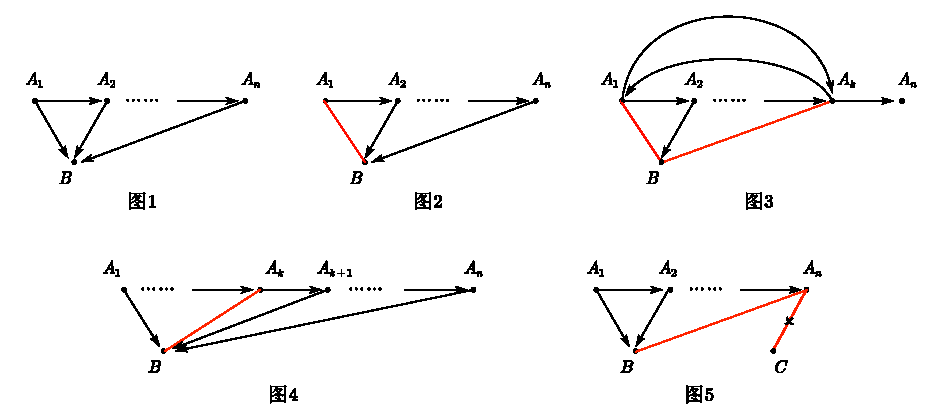
\includegraphics[width=16cm]{attachment/202302074.pdf}
	\end{center}
\end{solution}

\subsection{算两次}

\begin{problem} % 兴趣二阶组合3.1.1
	\nd{1}在$2006$张纸片的正面各写上整数$1$到$2006$中的一个,然后把纸片反过来弄乱,在纸片的反面同样写上整数$1$到$2006$中的一个.问:是否可能这$2006$张纸片的正反面上数的差(大数减小数)互不相同.
\end{problem}
\begin{solution}
	\begin{guess}
		若要满足这些差互不相同,所有的差应该是$0,1, \cdots ,2005$.若要产生$2005$,必须$2006-1$.同样地,为了产生$2004,2003, \cdots$,应该将两个数列交错排放,如下图所示:
		\begin{center}
			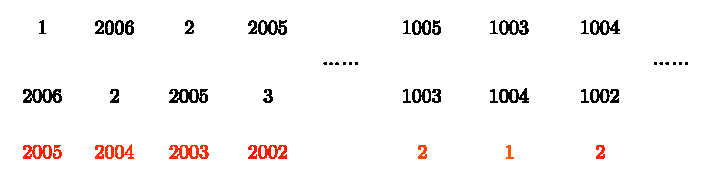
\includegraphics{attachment/202302081.pdf}
		\end{center}
		然而这种构造方法的问题在于它不会出现$0$,本质上就是“构造”的奇偶性与想要的奇偶性不同.
	\end{guess}
	容易发现,差$0, \cdots ,2005$的和是一个奇数. \\
	然而,由于$|a-b|$与$a+b$奇偶性相同,这些差之和的奇偶性与$2(1+ \cdots +2006)$应相同,意味着这些差之和是一个偶数,产生矛盾.故不可能找到互不相同的差.
\end{solution}

\begin{problem} % 兴趣二阶组合3.1.2,3.5
	\nd{1}(1)给定正奇数$n>1$.正$n$边形的顶点被三染色,且每种颜色的顶点恰有奇数个.证明:存在一个等腰三角形,其三个顶点两两不同色. \\
	(2)已知$R$为小于$2017$的正整数.一个正$2017$边形中恰有$R$个顶点为红色,其余顶点为蓝色.证明:三个顶点颜色相同的等腰三角形的个数不依赖于蓝色和红色顶点的分布.
\end{problem}
\begin{solution}
	(1)假设不存在这样的等腰三角形,因而所有的等腰三角形要么有$3$个同色边,要么有$1$个同色边与$2$个异色边.考虑二元组$(T,t)$的个数,其中$T$为等腰三角形,$t$为$T$中的异色边个数. \\
	一方面,对于$T$,每个等腰三角形都有偶数个异色边,故$(T,t)$有偶数个; \\
	另一方面,对于一个异色边对角线$t$,它总是在奇数个等腰三角形中(若$n$不是$3$的倍数,总能找到关于过其某一顶点平分多边形的直线对称的对角线,这会产生$2$个等腰三角形,以及以该对角线为底边的一个等腰三角形.当$n$为$3$的倍数时可以找到一个等边三角形),又$t$本身是奇数个,故$(T,t)$有奇数个.这产生矛盾,于是必然存在题目要求的等腰三角形. \\
	(2)记$A$为同色等腰三角形的个数,$B$为异色等腰三角形的个数.分别考虑$t$为同色边、异色边时$(T,t)$的个数(其中$T$表示等腰三角形),可知:
	$$3(C_R^2 + C_{2017-R}^2)=3A+B \qquad 3R(2017-R) = 2B$$
	解得$$A=C_R^2 + C_{2017-R}^2 - \dfrac{R(2017-R)}{2}$$
\end{solution}

\begin{problem} % 兴趣二阶组合3.3
	\nd{1}某委员会中共有$n$名委员,任意两名委员只能是朋友或敌人,每名委员恰有三个敌人.另外,对任意一名委员,他朋友的敌人均为他的敌人.求$n$的所有可能值.
\end{problem}
\begin{solution}
	首先,为了保证每名委员的敌人数不超过$3$,必须要求$n-3 \leq 3$,即$n \leq 6$. \\
	其次,考虑组$(A,B)$,其中$A,B$互为敌人.对于$A$,$(A,B)$共有$3n$个,而所有$(A,B)$的个数需要是偶数个(因为$(A,B)$与$(B,A)$是同种情况),于是有$$2~|~3n$$即$2~|~n$.这意味着$n=4~ \textit{或} ~6$.例如,如下的构造可以满足题目要求:
	\begin{center}
			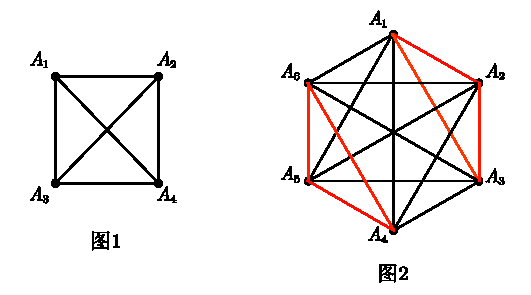
\includegraphics{attachment/202302082.pdf}
	\end{center}
\end{solution}

\begin{problem} % 兴趣二阶组合3.4
	\nd{1}设凸$n$边形($n \geq 4$)的任何$3$条对角线都不共点,求该多边形被它的所有对角线分成了多少块内部不相交的小多边形?
\end{problem}
\begin{solution}
	\begin{guess}
		先考虑一个简单的结论,如图$1$所示,当用$n$条直线划分一个平面时,若新增的直线可以被截为$m$段,而每一段将所在区域划为两块,那么这根直线就会产生$m$块区域.
	\end{guess}
	\begin{center}
			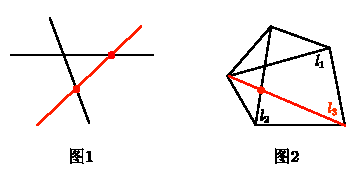
\includegraphics[width=7.5cm]{attachment/202302083.pdf}
	\end{center}
	如图$2$所示,依次连接$l_1, \cdots ,l_m$.每次新连接$l_k$时,设其与$l_1, \cdots ,l_{k-1}$交于$\alpha _k$个交点,那么将多分出$\alpha _k+1$块区域.于是总区域数为$$1 + (\alpha _1 +1) + \cdots + (\alpha _m + 1) = m+1 +(\alpha _1 + \cdots + \alpha _k)$$
	其中,由于$m=C_n^2-n$,$\alpha _1 + \cdots + \alpha _k = C_n^4$(因为一个(两条对角线产生的)交点可以由一个四边形唯一确定),可知总区域数为$$C_n^4+C_n^2-n+1 = \frac{n^4 - 6n^3 + 23n^2 - 42n + 22}{24}$$
\end{solution}

\begin{problem} % 兴趣二阶组合3.6
	在平面上有$n$条给定的直线($n \geq 3$),它们中的任意两条直线均不平行,且不存在三条直线共点,将这$n$条直线产生的所有的交点的集合记为$S$.求证:存在其中的一条直线,它将平面分成两个开区域,使得这两个开区域上的$S$中的交点个数均不小于$\left[ \dfrac{n^2-3n}{12} \right]$.
\end{problem}
\begin{solution}
	
\end{solution}


\chapter{兴趣二阶数论}

\begin{problem} % 兴趣二阶数论1.1
	黑板上写着五个正整数,其中任何三个数的和均可被其余两个数中的每一个整除.问:这五个数中是否一定有四个相同的数?
\end{problem}
\begin{solution}
	\begin{guess}
		设这五个数分别为$a,b,c,d,e$.对于$a$,由于$$a\mid b+c+d,\quad a\mid b+c+e,\quad a\mid b+d+e,\quad a\mid c+d+e$$
		可知$a\mid b-c,a\mid b-d,\cdots$.例如,对于$a\mid b-c$,为了让$b-c=0$,自然想到令$a$为最大元.
	\end{guess}
	不妨设这五个数分别为$a,b,c,d,e$,满足$a \geq b \geq c \geq d \geq e$.对于$a$,由于$a\mid b+d+e,~a\mid c+d+e$,故$a\mid b-c$.因为$b,c \leq a$,自然$b-c \leq a$,故$b-c=0$.同理$c-d=0,d-e=0$,即$b=c=d=e$.
\end{solution}

\begin{problem} % 兴趣二阶数论1.1
	已知正整数$n$有至少三个不同的真因子.求最小的$n$,使得这三个因子之和等于$1001$.
\end{problem}
\begin{solution}
	先求$n$的范围:容易发现,这三个真因子至多是$\dfrac{n}{2},\dfrac{n}{3},\dfrac{n}{4}$,可得$$1001 \leq \frac{n}{2} + \frac{n}{3} + \frac{n}{4}$$
	即$n \geq 924$.当$n=924$时,由于$462\mid n,308\mid n,231\mid n$,又$462+308+231=1001$,故原命题成立.
\end{solution}

\begin{problem} % 兴趣二阶数论1.2
	已知$13$分别除以$5,7,9$所得的余数依次为$3,6,4$,将三个余数相加仍然得到原数$13$. \\
	(1)设$a,b$均小于$n~(a,b,n \in \mathbb{Z}_+)$,证明:$n$除以$a,b$所得余数之和不可能等于$n$. \\
	(2)若$n~(n>229)$除以$99,132,229$所得余数之和仍为$n$,求所有的$n$.
\end{problem}
\begin{solution}
	(1)记$n=q_1a+r_1=q_2b+r_2$, \\
	当$a>\dfrac{n}{2}$时,$q_1=1$,因而$r_1<\dfrac{n}{2}$;当$a \leq \dfrac{n}{2}$时,总有$r_1 < a <\dfrac{n}{2}$.故$r_1<\dfrac{n}{2}$,同理$r_2<\dfrac{n}{2}$,于是$$r_1+r_2 < \frac{n}{2} + \frac{n}{2} = n$$
	即$r_1+r_2 \neq n$. \\
	(2)\begin{guess}
		注意到,$98+131=229$.自然想到$r \leq a-1$.
	\end{guess}
	设$n$除以$99,132,229$的余数分别为$r_1,r_2,r_3$,满足$n=r_1+r_2+r_3$.可知$$r_1 \leq 98,\quad r_2 \leq 131$$
	于是$r_1+r_2 \leq 229$.另一方面,由$229\mid n-r_3$,有$229 \leq n-r_3 \leq 229$,可知所有的等号全部取到,即$r_1=98,~r_2=131$,也即$$99\mid n+1,\quad 132\mid n+1$$
	再结合$229<n<229+228$(这是因为$n=r_1+r_2+r_3<229+228$),可知这样的$n$只有$395$一个.
\end{solution}

\begin{problem} % 兴趣二阶数论1.3
	设$a_1, \cdots ,a_{10}$是不小于$3$的互异正整数,满足$a_1+ \cdots + a_{10}=678$.是否存在正整数$n$,使得当$n$分别除以$a_1, \cdots ,a_{10},2a_1, \cdots ,2a_{10}$这$20$个数所得到的余数的和等于$2012$.
\end{problem}
\begin{solution}
	\begin{guess}
		记$n$除以$a_i,2a_i$的余数分别为$r_i,t_i$,对于$a_i$与$2a_i$,注意到$$r_i=\begin{cases}
			t_i-a_i &t_i \geq a_i \\
			t_i &t_i < a_i
		\end{cases},\quad i.e. \quad r_i+t_i=\begin{cases}
			2r_i+a_i<3a_i &t_i \geq a_i \\
			2r_i<2a_i &t_i < a_i
		\end{cases}$$
		由于$3(a_1+ \cdots + a_{10})$刚好超过$2012$,容易发现全都是第一种情况.
	\end{guess}
	记$n$除以$a_i,2a_i$的余数分别为$r_i,t_i$.由于
	\begin{align*}
		2012&=r_1+ \cdots + r_{10} + t_1 + \cdots + t_{10} \\
		&\leq (a_1-1)+ \cdots + (a_{10}-1)+(2a_1-1)+ \cdots + (2a_{10}-1) \\
		&=3(a_1+ \cdots + a_{10})-20=2014
	\end{align*}
	又因为$a_i \geq 3$,所以$t_i=a_i+r_i,~(i=1, \cdots ,10)$.代回上式,可得
	\begin{align*}
		2012 &= r_1+ \cdots + r_{10} + (a_1+r_1) + \cdots + (a_{10}+r_{10}) \\
		&= 2(r_1 + \cdots + r_{10}) + 678
	\end{align*}
	解得$r_1 + \cdots + r_{10}=667$.注意到,$r_1 + \cdots + r_{10} \leq a_1+ \cdots + a_{10}-10=668$,故必有唯一一个$a_m$使得$r_m+2=a_m$,即$2a_m\mid n+2$.又因为$2r_i\mid n+1~(i \neq m)$,而$n+1,n+2$中必有一个为奇数,故矛盾.
\end{solution}

\begin{problem} % 兴趣二阶数论1.4
	求所有满足下列条件的正整数$n$:(i)$n$至少含有$4$个正因子;(ii)对于$n$的任意正因子$a,b~(1<a<b<n)$,有$(b-a) \mid n$.
\end{problem}
\begin{solution}
	\begin{guess}
		容易发现,$n$在过大的时候会出问题,主要矛盾类似于“完美数”从第四项就开始变得巨大的原因,即素数在大数中分布不够密集.
	\end{guess}
	设$n$的正因子依次为$1<r_1< \cdots <r_k<n$.取$r_1,r_k$,可知$(r_k-r_1)\mid n$,即$$\ssb{ \frac{n}{r_1}-r_1 }\mid n$$
	因为$\ssb{ \dfrac{n}{r_1}-r_1 } \mid r_1\ssb{ \dfrac{n}{r_1}-r_1 }$,所以有$$\ssb{ \frac{n}{r_1}-r_1 }\mid r_1^2$$
	即$\ssb{ \dfrac{n}{r_1}-r_1}=1 \cor r_1 \cor r_1^2$.由此可解得$n=6 \cor 8 \cor 12$.
\end{solution}

\begin{problem} % 兴趣二阶数论1.5
	是否存在$2009$个不同的正整数满足其和被其中任意两个数的和整除?
\end{problem}
\begin{solution}
	\begin{guess}
		类似于上个问题,不妨设$a_1 < \cdots < a_{2009}$,$S=a_1+ \cdots + a_{2009}$,容易发现$\dfrac{S}{a_i+a_j} \in \mathbb{Z}$中的$a_i+a_j$分布比较均匀,然而$S$的因子在数比较大时应该稀疏.故寻找极值时的矛盾.
	\end{guess}
	假设存在这样的一组数$a_1, \cdots ,a_{2009}$,不妨设$a_1 < \cdots < a_{2009}$,$S=a_1+ \cdots + a_{2009}$,那么有$$2009 > \frac{S}{a_{2009}} > \frac{S}{a_1+a_{2009}} > \cdots > \frac{S}{a_{2008}+a_{2009}}$$
	由于该不等式链中每一项都是整数,可得$\dfrac{S}{a_{2008}+a_{2009}}=1$,于是$a_1+ \cdots + a_{2007}=0$,矛盾.综上,不存在这样的数.
\end{solution}

\begin{problem} % 兴趣二阶数论1.6
	求满足下列条件的正整数数对$(x,y)$:
	\begin{center}
		$(x+y+1) \mid 2xy,~(x+y-1) \mid (x^2+y^2-1)$
	\end{center}
\end{problem}
\begin{solution}
	\begin{guess}
		有一个操纵整除符号左边的结论:若$a \mid c,~b \mid c$,则$ab \mid c(a,b)$.
	\end{guess}
	由$(x+y-1) \mid (x^2+y^2-1)$,可得$(x+y-1) \mid 2(x+y-xy-1)$,那么$(x+y-1) \mid 2xy$. \\
	又$(x+y+1) \mid 2xy$,于是$$(x+y-1)(x+y+1) \mid 2xy (x+y-1,x+y+1)$$
	其中,$(x+y-1,x+y+1)=(x+y-1,2)=1\cor 2$. \\
	\buzhou{1} 当$(x+y-1,x+y+1)=1$时,即有$$(x+y)^2-1 \mid 2xy,\quad i.e.~(x+y)^2-1 \leq 2xy$$可得$x^2+y^2 \leq 1$.因为$x,y$均为正整数,$(x,y)$无解; \\
	\buzhou{2} 当$(x+y-1,x+y+1)=2$时,即有$$(x+y)^2-1 \mid 4xy,\quad i.e.~(x+y)^2-1 \leq 4xy$$可得$(x-y)^2 \leq 1$.若$x=y$,代入上式,则$4x^2-1 \mid 4x^2$,显然不成立;若$y=x+1$,经验证符合条件;同理,若$x=y+1$,也符合条件. \\
	综上,满足要求的$(x,y)$为$(k,k+1)$及$(k+1,k)$,其中$k$为正整数.
\end{solution}

\begin{problem} % 兴趣二阶数论1.7
	求所有的正整数对$(a,b)$,使得$a^2b \mid b^2+3a$.
\end{problem}
\begin{solution}
	由$a^2b \mid b^2+3a$,有$b \mid b^2+3a$,于是$b \mid 3a$. \\
	\buzhou{1} 若$(b,3)=1$,则$b \mid a$.令$a=kb$,则$k^2b^3 \mid (3k+b)b$,于是$k^2b^2 \mid 3k+b$,可得$k^2b^2 \leq 3k+b$. \\
	(i)~若$k \geq b$,那么$k^2b^2 \leq 4k$,于是$kb^2 \leq 4$.只能$b=1$,即有$k^2 \mid 3k+1,~k^2 \leq 3k+1$,解得$k=1$.此时即$(a,b)=(1,1)$; \\
	(ii)~若$k \leq b$,那么$k^2b^2 \leq 4b$,于是$k^2b \leq 4$.只能$k=1$,即有$b^2 \mid b+3,~b^2 \leq b+3$,解得$b=1\cor 2$.然而这两个解均不成立,故此时无解. \\
	\buzhou{2} 若$(b,3)=3$,令$b=3b_1$,于是$b_1 \mid a$.设$a=l b_1$,同\buzhou{1}可知$l=b_1=1$,即$(a,b)=(1,3)$时可行. \\
	综上,满足条件的整数对为$(1,1),~(1,3)$.
\end{solution}

\begin{problem} % 兴趣二阶数论1.8
	求出所有的正整数$x,y,p,n,k$,满足$\begin{cases}
		5x+y=p^k \\ 5y+x=p^{n+k}
	\end{cases}$.
\end{problem}
\begin{solution}
	将方程组视作关于$x,y$的,得$x=\dfrac{p^k \cdot (5-p^n)}{24},~y=\dfrac{p^k \cdot (5p^n-1)}{24}$. \\
	由于$x,y>0$,可知$\dfrac{1}{5} < p^n < 5$.另外,当$p^n=1$时,有$5x+y=1$,矛盾,故$p^n=2,3,4$. \\
	\buzhou{1} 若$p^n=2$,必有$p=2,~n=1$.此时$x=\dfrac{2^k}{8},~y=\dfrac{3 \cdot 2^k}{8}$.只需$k \geq 3$即可符合题意. \\
	\buzhou{2} 若$p^n=3$,必有$p=3,~n=1$.此时$x=\dfrac{3^k}{12},~y=\dfrac{7 \cdot 3^k}{12}$,$y$一定不是整数,故此时无解. \\
	\buzhou{3} 若$p^n=4$,则$x=\dfrac{p^k}{24}$.由于此时$p=2\cor 4$,$x$一定不是整数,故此时无解. \\
	综上,满足条件的整数对为$(x,y,p,n,k)=(2^{k-3},3\cdot 2^{k-3},2,1,k)$,其中$k \geq 3$.
\end{solution}

\begin{problem} % 兴趣二阶数论1.9
	对于自然数$N$,记$N$的标准分解式为$N=p_1^{\alpha _1}p_2^{\alpha _2} \cdots p_n^{\alpha _n}$,其中,$p_i$为两两不同的素数,$a_i \in \mathbb{Z}_{+},~a \leq i \leq n$.记$T(N)=a_1+a_2+ \cdots + a_n$. \\
	已知四个不同的自然数$a,b,c,d$满足$(ac+bd) \mid (ab+cd)$.证明:$T(ab+cd) \geq 3$.
\end{problem}
\begin{solution}
	\begin{guess}
		当$T(ab+cd)$比较小时会好想一点,考虑用反证法.
	\end{guess}
	假设$T(ab+cd) \leq 2$. \\
	\buzhou{1} 若$T(ab+cd)=1$,即$ab+cd$为素数.由$(ac+bd) \mid (ab+cd)$,$ac+bd=1\cor ab+cd$.又$a,b,c,d$为不同的自然数,$ac+bd=ab+cd$,于是$(a-d)(c-b)=0$,总存在两个相等的数,矛盾. \\
	\buzhou{2} 若$T(ab+cd)=2$,记$ab+cd=p_1p_2$.若$ab+cd=ac+bd$,由\buzhou{1}可知这样会产生矛盾.故不妨令$ac+bd=p_1$.由$\dfrac{ab+cd}{ac+bd} \in \mathbb{Z}$,有$\dfrac{(a+d)(b+c)}{p_1} \in \mathbb{Z}$.不妨令$ac+bd \mid a+d$,于是$b=c=1$,矛盾. \\
	综上,$T(ab+cd) \geq 3$.
\end{solution}

\begin{problem} % 兴趣二阶数论2.1
	对于任意的整数$n \geq k$,证明:$C_n^k,C_{n+1}^k, \cdots ,C_{n+k}^{k}$的最大公约数等于$1$.
\end{problem}


\end{document}
